\setchapterstyle{kao}
\setchapterpreamble[u]{\margintoc}
\chapter{Doce de Laranja}\label{doce de laranja}

\section{Ingredients}

\begin{multicols}{2}
	\begin{description}
		\item[$1\times$] Orange juicy oranges
		\item[$0.5\times$] Crystal sugar
		\item[Some] Cryatal sugar for coating
	\end{description}
\end{multicols}	

\section{Preparation}
First, weight out your oranges. The amount of sugar is half of the weight of the oranges.

Squeeze the juice out of the oranges, and reserve it, we will use it latter. Remove the ending of the oranges as they are a bit ticker, and for not clean the bits nor the white part of the skin.

Boil the skin $3\times$, for $15~min$ each time, changing the water. In the end the skins should be very soft.

After that, add the oranges skin to a wide pan with the sugar and the juice, and boil it until water vapor stops coming out, and when the first, ever so slight, note of caramel hits your nose. We do not want to caramelize this.\sidenote{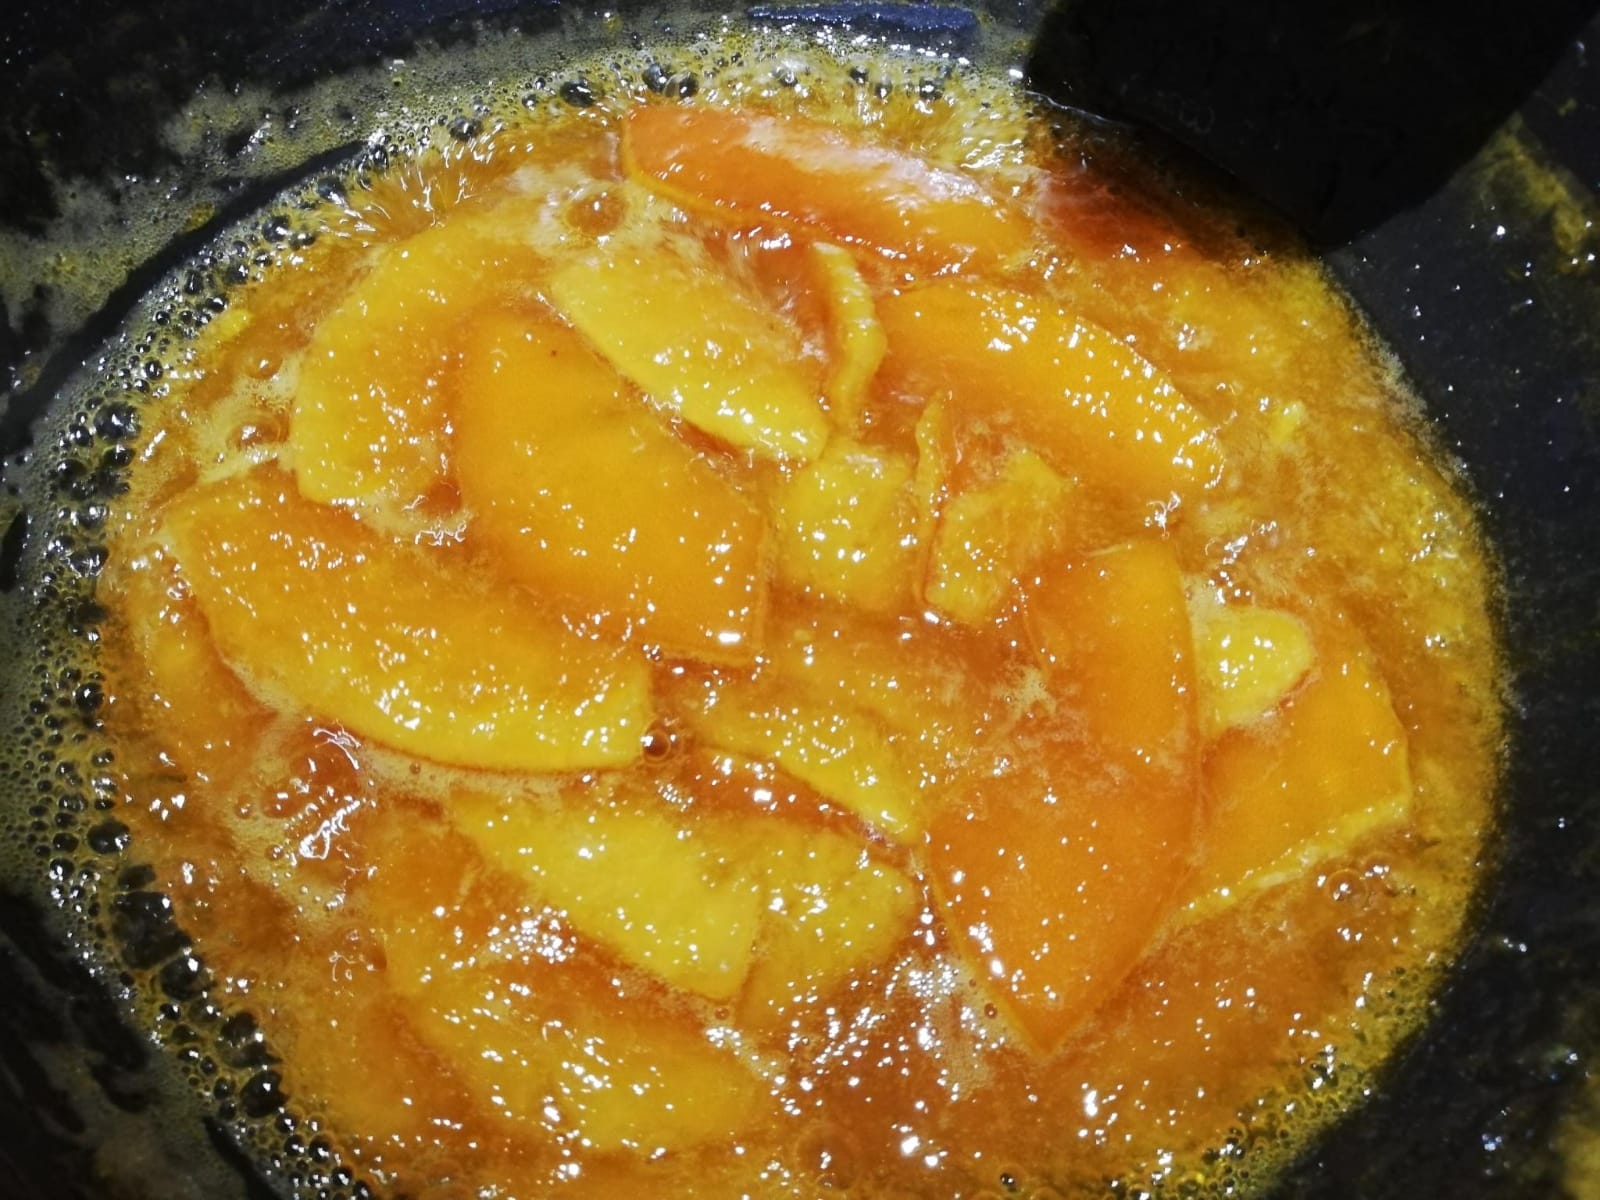
\includegraphics{images/doce-de-laranja1}}

Dry the skins in a rack for a day\sidenote{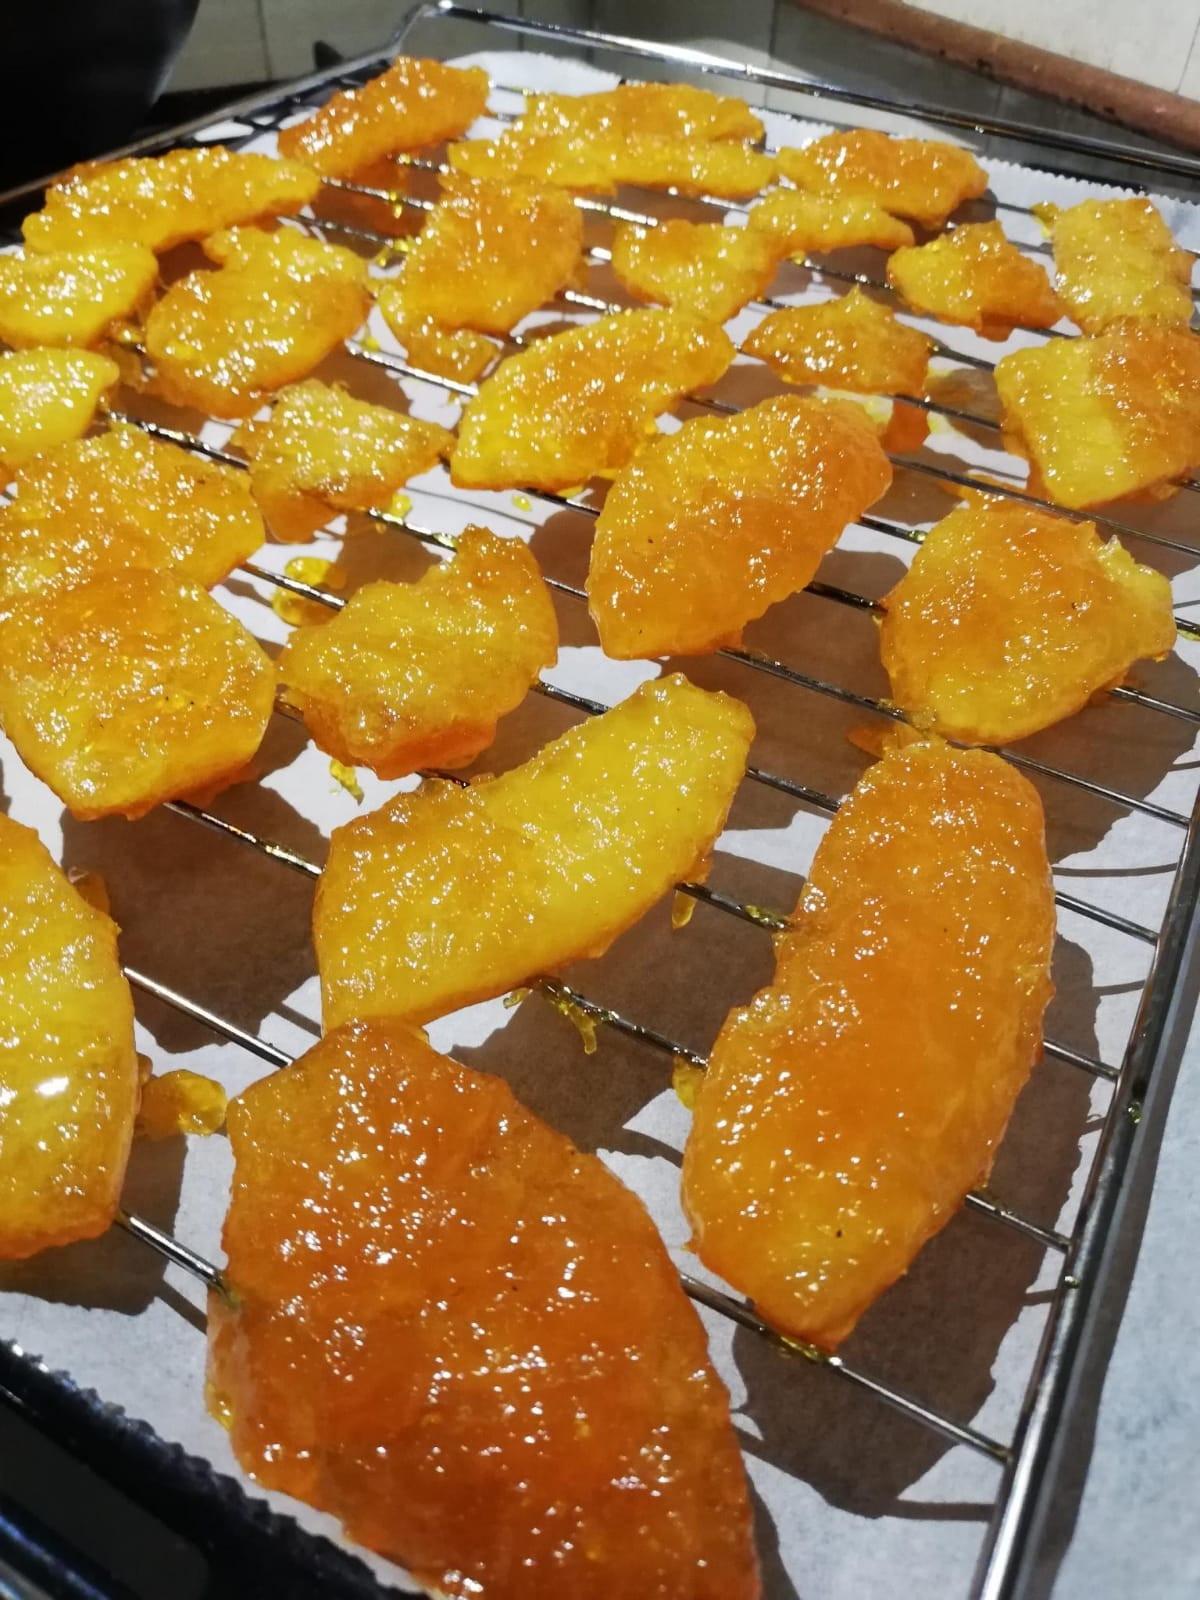
\includegraphics{images/doce-de-laranja2}}, then cover them in sugar. Preserve in a container by layering then with sugar.

\section{Usage}
Biscuits, panettone, thin slices coated with chocolate are traditional. Be creative.
